\chapter{Introdução}
%%
%% Capítulo 1: Modelo de Capítulo
%%

% Está sendo usando o comando \mychapter, que foi definido no arquivo
% comandos.tex. Este comando \mychapter é essencialmente o mesmo que o
% comando \chapter, com a diferença que acrescenta um \thispagestyle{empty}
% após o \chapter. Isto é necessário para corrigir um erro de LaTeX, que
% coloca um número de página no rodapé de todas as páginas iniciais dos
% capítulos, mesmo quando o estilo de numeração escolhido é outro.
\paragrafo{}
Texto Texto Texto Texto Texto Texto Texto Texto Texto Texto Texto Texto Texto Texto Texto Texto Texto Texto Texto Texto Texto Texto Texto Texto Texto Texto Texto Texto Texto Texto Texto Texto Texto Texto Texto Texto Texto Texto Texto Texto Texto Texto. 
\section{Apresentação}
\label{apresentacao}
\paragrafo{}
Texto Texto Texto Texto Texto Texto Texto Texto Texto Texto Texto Texto Texto Texto Texto Texto Texto Texto Texto Texto Texto Texto Texto Texto Texto Texto Texto Texto Texto Texto Texto Texto Texto Texto Texto Texto Texto Texto Texto Texto Texto Texto. 
\paragrafo{}
Texto Texto Texto Texto Texto Texto Texto Texto Texto Texto Texto Texto Texto Texto Texto Texto Texto Texto Texto Texto Texto Texto Texto Texto Texto Texto Texto Texto Texto Texto Texto Texto Texto Texto Texto Texto Texto Texto Texto Texto Texto Texto. 
\section{Objetivos}
\label{objetivo}
\subsection{Objetivo Geral}
\paragrafo{}
Texto Texto Texto Texto Texto Texto Texto Texto Texto Texto Texto Texto Texto Texto Texto Texto Texto Texto Texto Texto Texto Texto Texto Texto Texto Texto Texto Texto Texto Texto Texto Texto Texto Texto Texto Texto Texto Texto Texto Texto Texto Texto.
\subsection{Objetivos Específicos}

\begin{itemize}
  \item \textbf{Objetivo específico 1} : Texto Texto Texto Texto Texto Texto Texto Texto Texto Texto Texto Texto Texto.
  \item \textbf{Objetivo específico 2} : Texto Texto Texto Texto Texto Texto Texto Texto Texto Texto Texto Texto Texto.
  \item \textbf{Objetivo específico 3} : Texto Texto Texto Texto Texto Texto Texto Texto Texto Texto Texto Texto Texto.
\end{itemize}
\section{Justificativa}
\label{justificativa}
\paragrafo{}
Texto Texto Texto Texto Texto Texto Texto Texto Texto Texto Texto Texto Texto Texto Texto Texto Texto Texto Texto Texto Texto Texto Texto Texto Texto Texto Texto Texto Texto Texto Texto Texto Texto Texto Texto Texto Texto Texto Texto Texto Texto Texto.
\paragrafo{}
Texto Texto Texto Texto Texto Texto Texto Texto Texto Texto Texto Texto Texto Texto Texto Texto Texto Texto Texto Texto Texto Texto Texto Texto Texto Texto Texto Texto Texto Texto Texto Texto Texto Texto Texto Texto Texto Texto Texto Texto Texto Texto.

\section{Estrutura dos Capítulos}
\label{estrutura}
\paragrafo{}
Texto Texto Texto Texto Texto Texto Texto Texto Texto Texto Texto Texto Texto Texto Texto Texto Texto Texto Texto Texto Texto Texto Texto Texto Texto Texto Texto Texto Texto Texto Texto Texto Texto Texto Texto Texto Texto Texto Texto Texto Texto Texto.
\paragrafo{}
Texto Texto Texto Texto Texto Texto Texto Texto Texto Texto Texto Texto Texto Texto Texto Texto Texto Texto Texto Texto Texto Texto Texto Texto Texto Texto Texto Texto Texto Texto Texto Texto Texto Texto Texto Texto Texto Texto Texto Texto Texto Texto.
\paragrafo{}
Texto Texto Texto Texto Texto Texto Texto Texto Texto Texto Texto Texto Texto Texto Texto Texto Texto Texto Texto Texto Texto Texto Texto Texto Texto Texto Texto Texto Texto Texto Texto Texto Texto Texto Texto Texto Texto Texto Texto Texto Texto Texto.
 \begin{figure}[H]
    \begin{center}
      % fbox faz uma borda ao redor do seu argumento
		\legenda{Exemplo de Imagem com Latex}
		\fbox{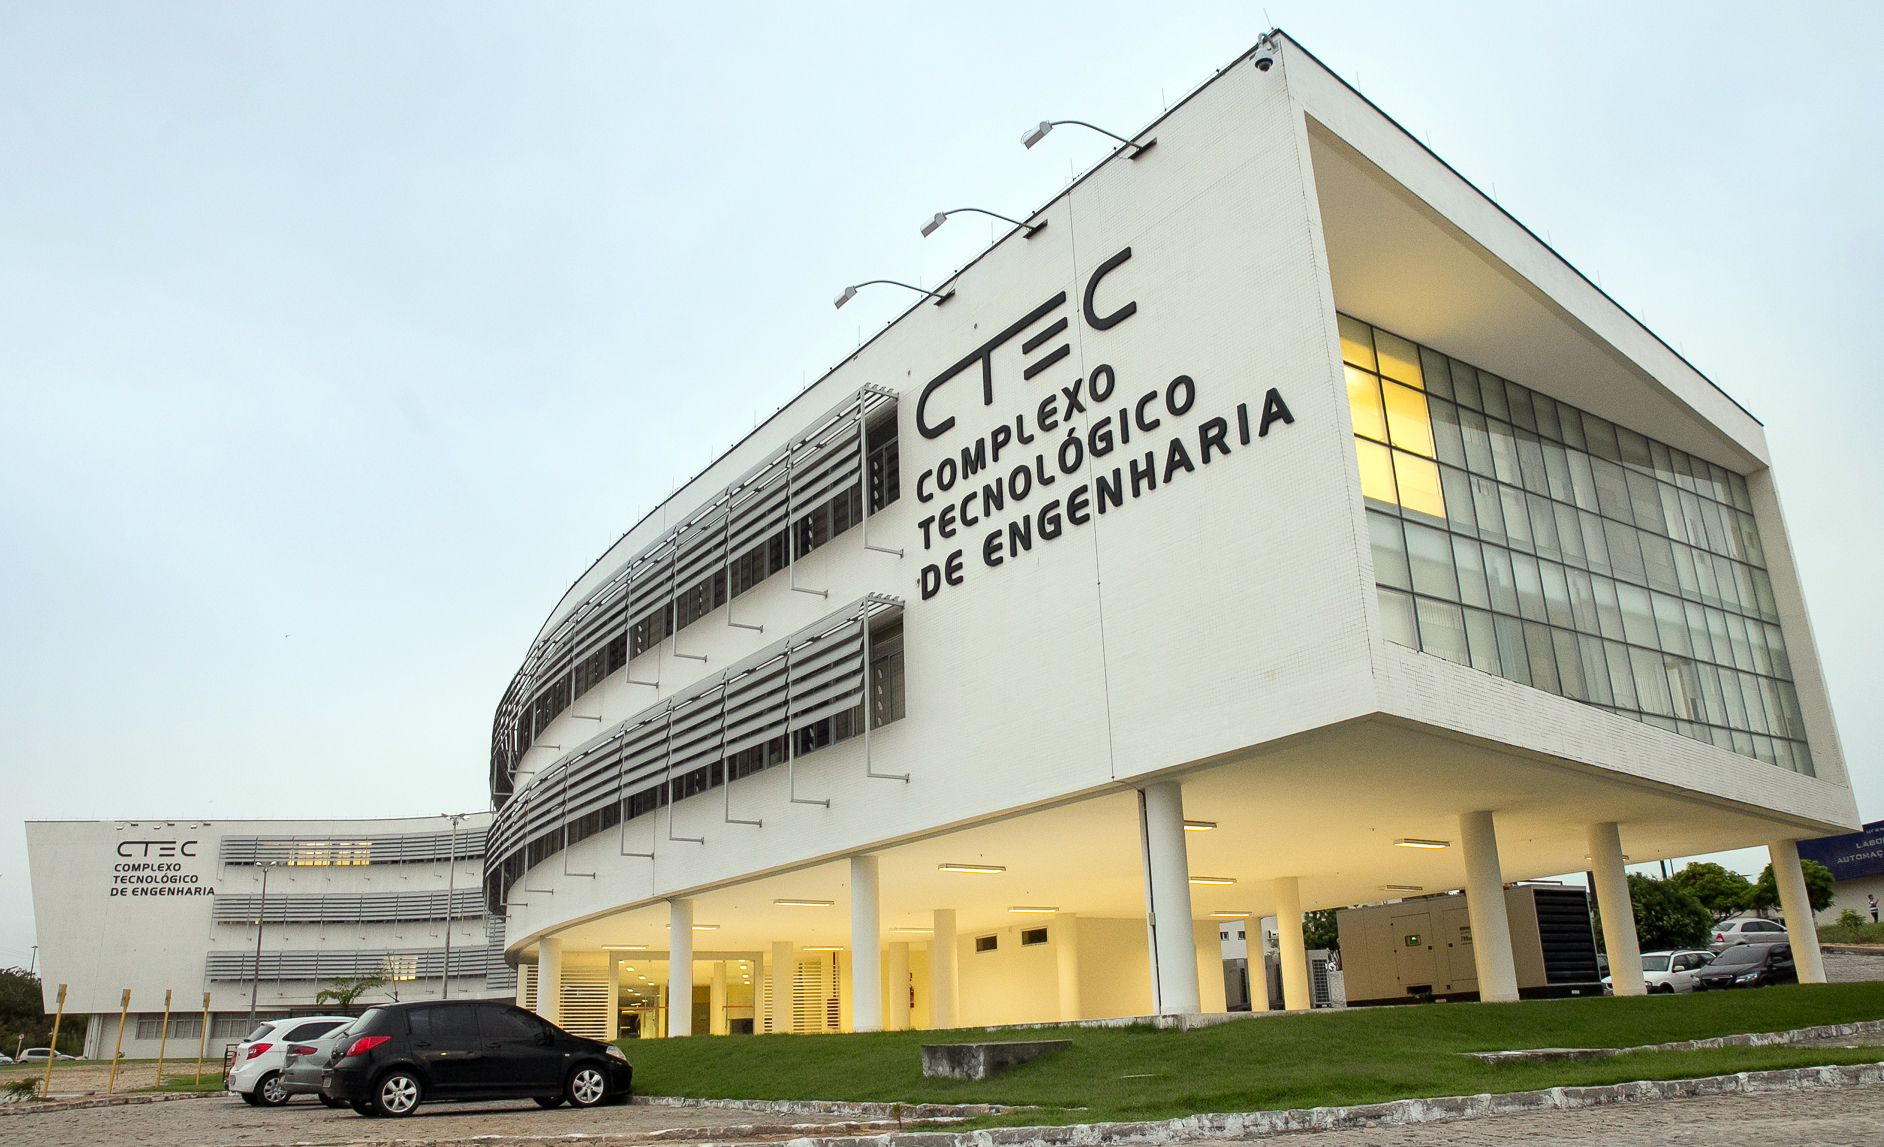
\includegraphics[width=0.95\linewidth]{internos/textuais/capitulo1-introducao/figuras/ctec.jpg}}
		\source{Internet}
		\label{Fig:exemplo1}
	\end{center}
\end{figure}
